\subsection{Problem Formulation}
There are many elements that affect location selection for charging stations when operators make the decision. In this paper, we hold that use rate of a station is the key factor which determines the 'success' of the station. Therefore, the original problem turns into how to get a higher use rate and what are the factors behind it. 

The main objectives of our work is three-fold. First, we aim to explore some important featrues that have great impact on use rate of a station using spatio-temporal data of operator's charging station data. Second, we propose to study stations' different 'behaviours' during diverse time frames. Finally, on the basis of time frame based framework, we aim to predict that one station is of high use rate or low use rate according to its georaphical information and working elements during different time periods.

\subsection{Design Methodology}
Since we consider that diffrent features may have different influence on station's use rate, we make detailed analyses on features like geographical information and stations' working elements. Furthermore, station's use rate may differ during different time periods, so that we also study on each time frame to find the changes. Based on all the analyses mentioned above, we propose the time frame based framework to help with use rate prediction for charging stations. We then apply three machine learning algorithms including SVC, Random Forest and MLP(ANN) to implement our experiments on different area districts and time frames. Fig.\ref{fig2} gives the overall data processing and learning pipelines of our work.

\begin{figure*}[!htp]
	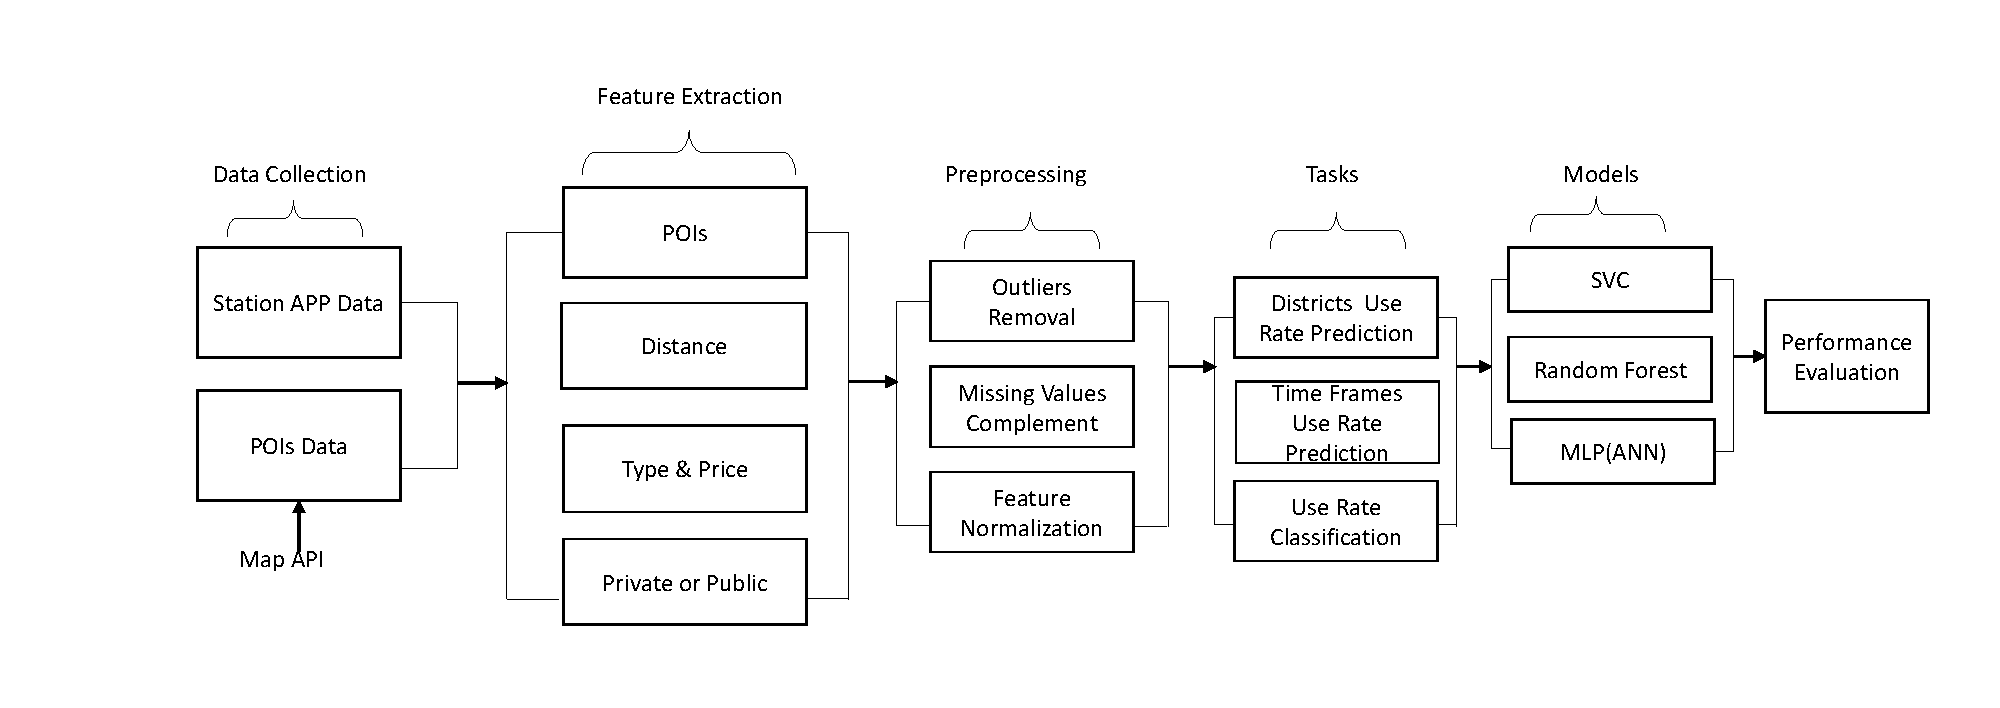
\includegraphics[width=2\columnwidth]{./figures/pipeline.pdf}
	\centering
	\caption{Overall Pipelines of Data Processing and Learning}
	\label{fig2}
\end{figure*}
